
\FloatBarrier

\section{Swedish Leaves}

\begin{figure}
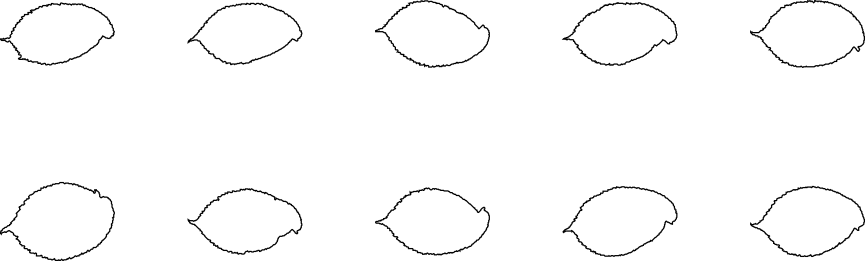
\includegraphics[width=0.45\linewidth]{experiments/0.datasets/leaves/output.d/leaves_01.png}
\hfill
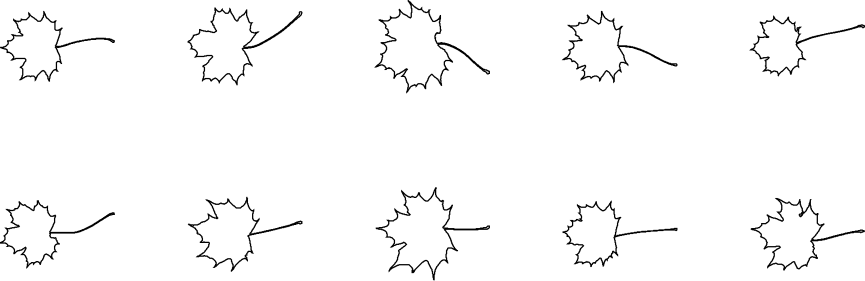
\includegraphics[width=0.45\linewidth]{experiments/0.datasets/leaves/output.d/leaves_02.png}
\\\vspace{3\baselineskip}
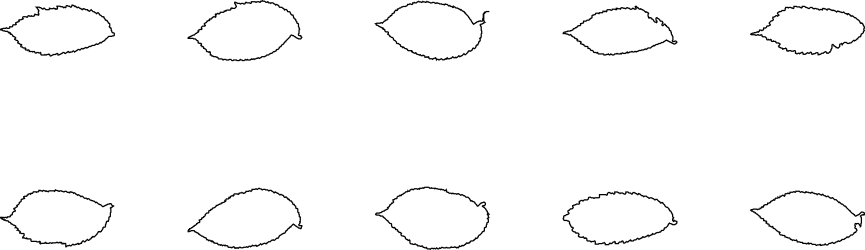
\includegraphics[width=0.45\linewidth]{experiments/0.datasets/leaves/output.d/leaves_03.png}
\hfill
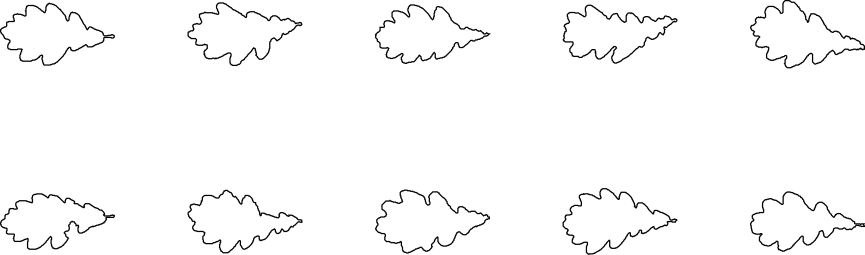
\includegraphics[width=0.45\linewidth]{experiments/0.datasets/leaves/output.d/leaves_04.png}
\\\vspace{3\baselineskip}
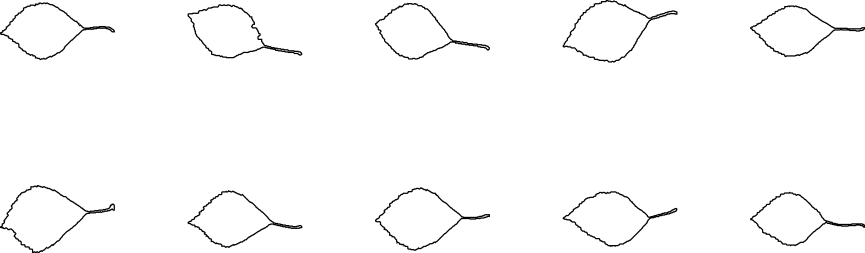
\includegraphics[width=0.45\linewidth]{experiments/0.datasets/leaves/output.d/leaves_05.png}
\hfill
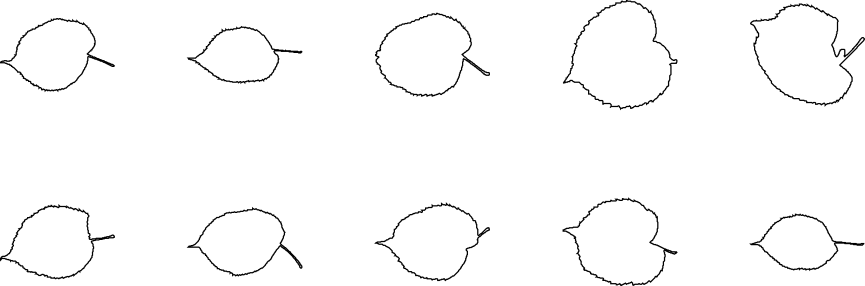
\includegraphics[width=0.45\linewidth]{experiments/0.datasets/leaves/output.d/leaves_06.png}
\\\vspace{3\baselineskip}
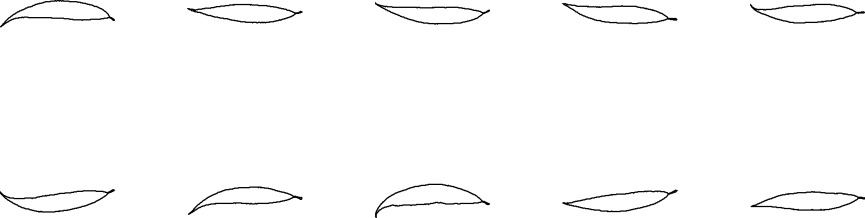
\includegraphics[width=0.45\linewidth]{experiments/0.datasets/leaves/output.d/leaves_07.png}
\hfill
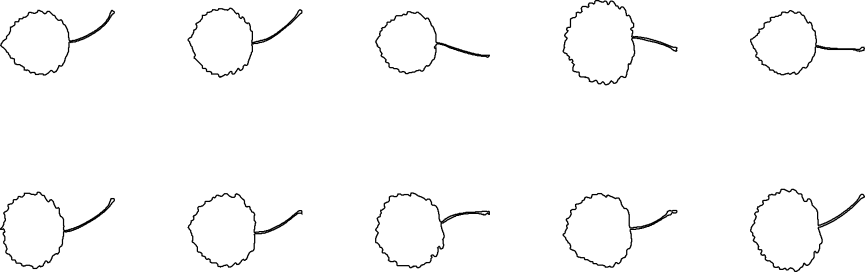
\includegraphics[width=0.45\linewidth]{experiments/0.datasets/leaves/output.d/leaves_08.png}
\\\vspace{3\baselineskip}
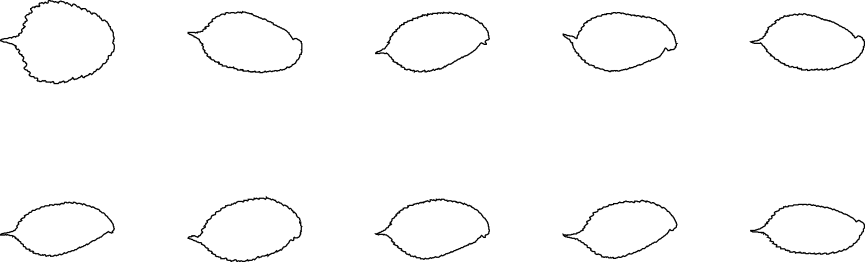
\includegraphics[width=0.45\linewidth]{experiments/0.datasets/leaves/output.d/leaves_09.png}
\hfill
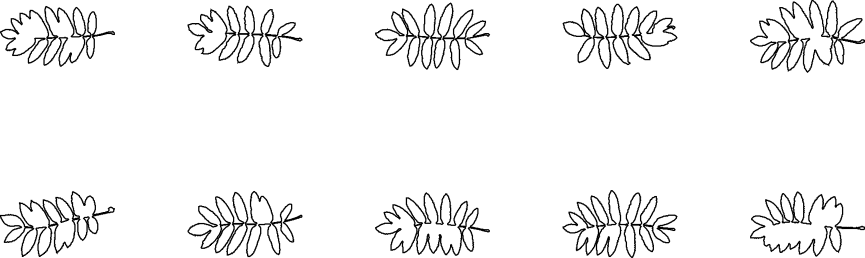
\includegraphics[width=0.45\linewidth]{experiments/0.datasets/leaves/output.d/leaves_10.png}
\\\vspace{3\baselineskip}
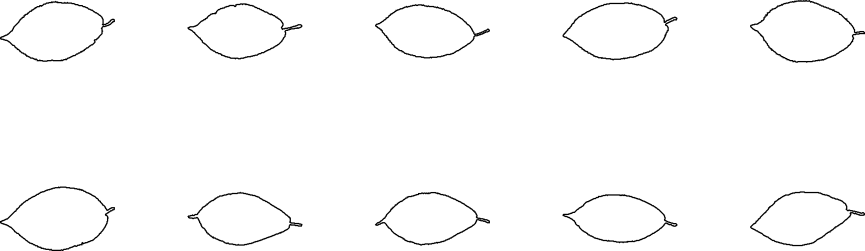
\includegraphics[width=0.45\linewidth]{experiments/0.datasets/leaves/output.d/leaves_11.png}
\hfill
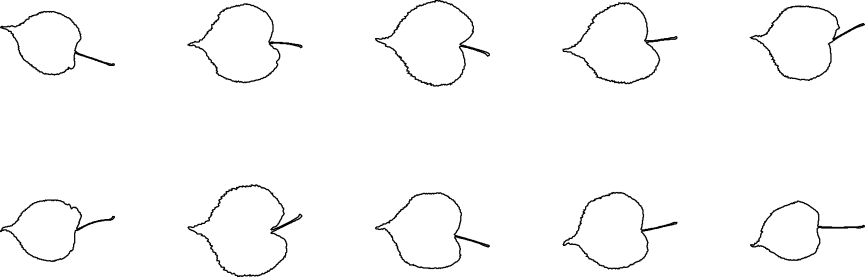
\includegraphics[width=0.45\linewidth]{experiments/0.datasets/leaves/output.d/leaves_12.png}
\\\vspace{3\baselineskip}
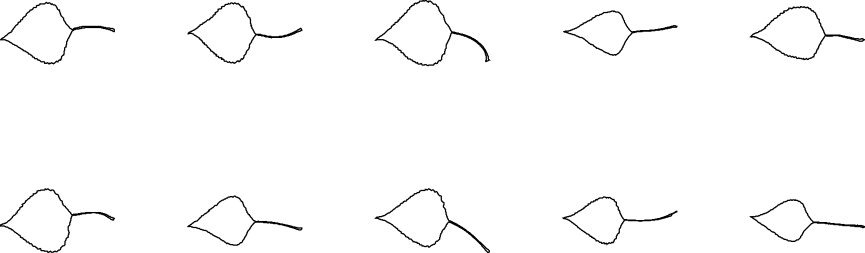
\includegraphics[width=0.45\linewidth]{experiments/0.datasets/leaves/output.d/leaves_13.png}
\hfill
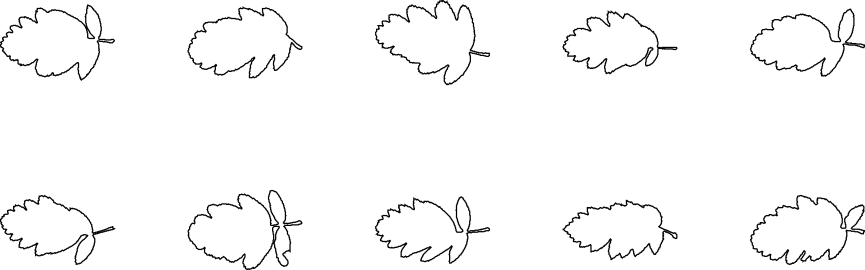
\includegraphics[width=0.45\linewidth]{experiments/0.datasets/leaves/output.d/leaves_14.png}
\\\vspace{3\baselineskip}
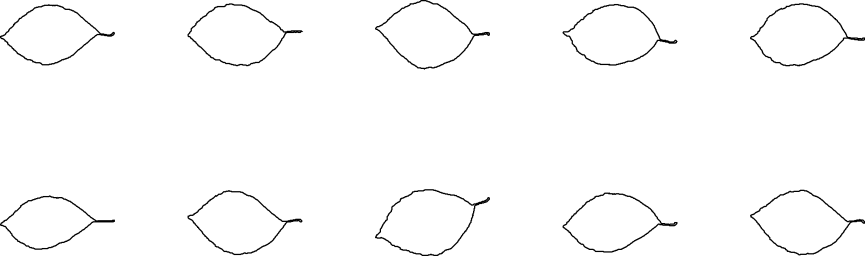
\includegraphics[width=0.45\linewidth]{experiments/0.datasets/leaves/output.d/leaves_15.png}
\caption{Swedish leaf dataset. The task is to distinguish between different species of tree by the shape of their leaves. There are 15 classes and 75 examples in each class.}
\end{figure}